\documentclass{article}

\usepackage[a4paper]{geometry}
\usepackage[ngerman]{babel}
\usepackage[utf8]{inputenc}
\usepackage[T1]{fontenc}
\usepackage{tabularx}
\usepackage{graphicx}

\graphicspath{ {./images/} }

\begin{document}

\begin{titlepage}
	\begin{flushleft}
		TH Brandenburg \\
		Online Studiengang Medieninformatik \\
		Fachbereich Informatik und Medien \\
		Mensch-Computer-Interaktion \\
		Prof. Dr. Martin Christof Kindsmüller
	\end{flushleft}

	\vfill

	\begin{center}
		\Large{Einsendeaufgabe 1: Personas und Storyboards}\\[0.5em]
		\large{Sommersemester 2021}\\[0.25em]
		\large{Abgabetermin 18.04.2021}
	\end{center}

	\vfill

	\begin{flushright}
		Maximilian Schulke \\
		Matrikel-Nr. 20215853
	\end{flushright}
\end{titlepage}

\tableofcontents

\vfill

\section{Aufgabenstellung}

Folgende Aufgabenstellung wurde im Moodle-Kurs bekannt gegeben:

\begin{quote}
	Sie haben die Aufgabe eine Smartphone-App zu konzipieren, die OSMI-Studierende beim Studium unterstützt.
	Die App soll insbesondere die Kommunikation, die gegenseitige Unterstützung und das gemeinsame Bearbeiten
	von Aufgaben und Projekten unterstützen. Denken Sie auch darüber nach, wie die App in der aktuellen
	SARS-CoV-2-Situation helfen kann (also beispielsweise auch Studierende, die normalerweise in Präsenz studieren).
	\\[1em]
	(a) Erstellen Sie zwei Personas der (potentiellen) Zielgruppe.

	(b) Erstellen Sie für jede Persona zwei Storyboards (also insgesamt vier) zur Nutzung der App. Storyboards
	werden in der Regel von Hand gezeichnet (auf Schönheit kommt es in diesem Zusammenhang nicht an). Scannen
	oder fotografieren Sie die Skizzen und beschreiben Sie ggf. kurz wie die Skizzen verstanden werden sollen.
	\\[1em]
	Anmerkungen:

	Abzugeben ist ein PDF-Dokument, das Ihre Ausführungen enthält. Bitte beachten Sie dazu die Hinweise zu den
	Einsendeaufgaben (siehe oben). Der zeitliche Umfang dieser Einsendeaufgabe wird auf 6 Stunden geschätzt.
	Ihre Ausarbeitung sollte ca. 7-9 Seiten (A4) umfassen (eine Seite für Titelblatt inkl. Aufgabenstellung,
	je eine Seite pro Persona, und je eine pro Storyboard sowie ggf. zusätzliche Seiten für die Erläuterungen).
	Die Lösung, die Sie zur Deadline abgeben, sollte eine aus Ihrer Sicht endgültige Lösung sein. Falls Sie
	Fragen zur Aufgabenstellung haben, stellen Sie diese bitte im Vorfeld!
\end{quote}

\newpage

\section{Personas}

\subsection{Mark Zahn}

\begin{figure}[h]
	
\includegraphics[width=0.25\textwidth]{mark}
	\centering
	\caption{Portrait von ``Mark Zahn`` (Roman Holoschchuk, unsplash.com)}
\end{figure}

\begin{quote}
	\large{``Ich verbringe meine Zeit gerne mit meiner Familie. Wenn ich Abends noch studiere, dann versuche
		ich möglichst effizient durch den Stoff zu kommen. Bisher habe ich eher selten in Lerngruppen gearbeitet,
		da mir der Austausch mit anderen Studenten immer sehr Zeitaufwendig vorkam.``}
\end{quote}

\begin{center}
	\begin{tabularx}{\textwidth}{|l|X|}
		\hline
		\textbf{Demographische Daten} &                                                     \\
		\hline
		Name                          & Marc Zahn                                           \\
		\hline
		Alter                         & 28                                                  \\
		\hline
		Beruf                         & Hochschul-Verwaltungsangestellter                   \\
		\hline
		Bildungsabschluss             & Abitur                                              \\
		\hline
		Familienstand                 & Verheiratet                                         \\
		\hline
		Kinder                        & Ja                                                  \\
		\hline
		Wohnort                       & Brandenburg an der Havel                            \\
		\hline
		\textbf{Persönlichkeit}       &                                                     \\
		\hline
		Motivation für OSMI           & Möchte nun Umlernen, bekam Kontakt zum OSMI als
		Umschulungsmöglichkeit, durch seinen Job an einer Hochschule                        \\
		\hline
		Hobbies                       & Alte Filme sammeln, Kochen, Wandern                 \\
		\hline
		OSMI-Student seit             & WS 2019                                             \\
		\hline
		Bedürfnisse                   & Erfolg, Soziale Anerkennung, Sicherheit für Familie \\
		\hline
		Wünsche                       & Neuer Job in Wunschbereich                          \\
		\hline
		Werte                         & Treue, Zuverlässigkeit, Ehrlichkeit                 \\
		\hline
		Ängste                        & Angst zu Versagen, Unsichere Zukunft                \\
		\hline
		Persönlichkeitstyp            & Introvertiert                                       \\
		\hline
	\end{tabularx}
\end{center}

\newpage

\subsection{Rosa Beetz}

\begin{figure}[h]
	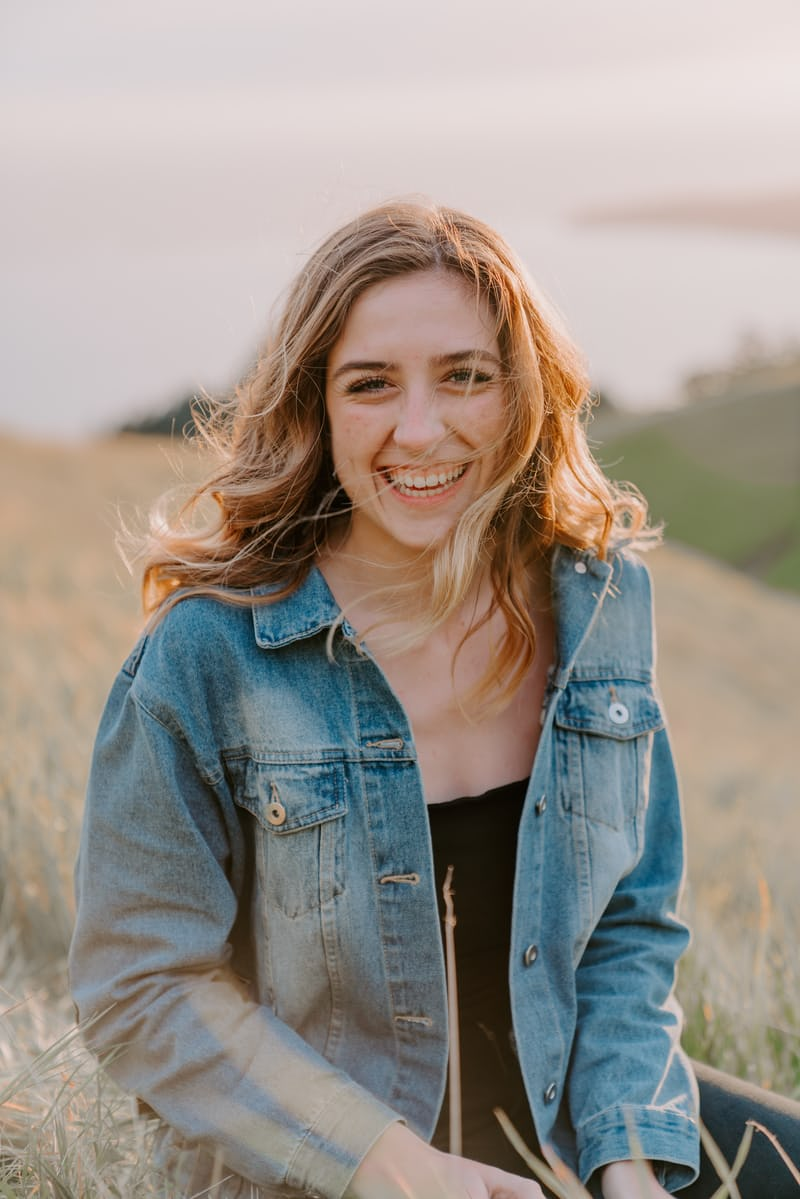
\includegraphics[width=0.25\textwidth]{rosa}
	\centering
	\caption{Portrait von ``Rosa Beetz`` (Svyatoslav Romanov, unsplash.com)}
\end{figure}

\begin{quote}
	\large{``Ich bin gerne mit anderen Menschen zusammen und finde, dass das Studium
		zusammen viel mehr Spaß macht und man besser lernt. Deshalb habe ich mit einigen
		Kommilitonen eine Lerngruppe gegründet.``}
\end{quote}

\begin{center}
	\begin{tabularx}{\textwidth}{|l|X|}
		\hline
		\textbf{Demographische Daten} &                                                     \\
		\hline
		Name                          & Rosa Beetz                                          \\
		\hline
		Alter                         & 23                                                  \\
		\hline
		Beruf                         & Screen Desginerin                                   \\
		\hline
		Bildungsabschluss             & Ausbildung                                          \\
		\hline
		Familienstand                 & Ledig                                               \\
		\hline
		Kinder                        & Nein                                                \\
		\hline
		Wohnort                       & Berlin Wedding                                      \\
		\hline
		\textbf{Persönlichkeit}       &                                                     \\
		\hline
		Motivation für OSMI           & Möchte sich in Richtung Informatik weiterentwickeln
		und sich selbst etwas Beweisen                                                      \\
		\hline
		Hobbies                       & Netflix, Feiern, guter Kaffee \& Kreativität        \\
		\hline
		OSMI-Student seit             & SS 2021                                             \\
		\hline
		Bedürfnisse                   & Sozialer Kontakt, Anerkennung                       \\
		\hline
		Wünsche                       & Mehr Geld, Anerkennung im Job                       \\
		\hline
		Werte                         & Freundlichkeit, Ehrgeiz                             \\
		\hline
		Ängste                        & Angst zu Versagen                                   \\
		\hline
		Persönlichkeitstyp            & Extrovertiert                                       \\
		\hline
	\end{tabularx}
\end{center}

\newpage

\section{Storyboards}

\subsection{Storyboard 1 für Mark Zahn}

\begin{figure}[h]
	
\includegraphics[angle=90,width=\textwidth]{mark}
	\centering
	\caption{Storyboard Mark – Als OSMI Studen möchte ich xyz}
\end{figure}

\newpage

\subsection{Storyboard 2 für Mark Zahn}

\begin{figure}[h]
	
\includegraphics[angle=90,width=\textwidth]{mark}
	\centering
	\caption{Storyboard Mark – Als OSMI Student möchte ich unkompliziert mit anderen Studenten in einer PDF zusammenarbeiten, um den Zeitaufwand der Zusammenarbeit zu minimieren.}
\end{figure}

\newpage

\subsection{Storyboard 3 für Rosa Beetz}

\begin{figure}[h]
	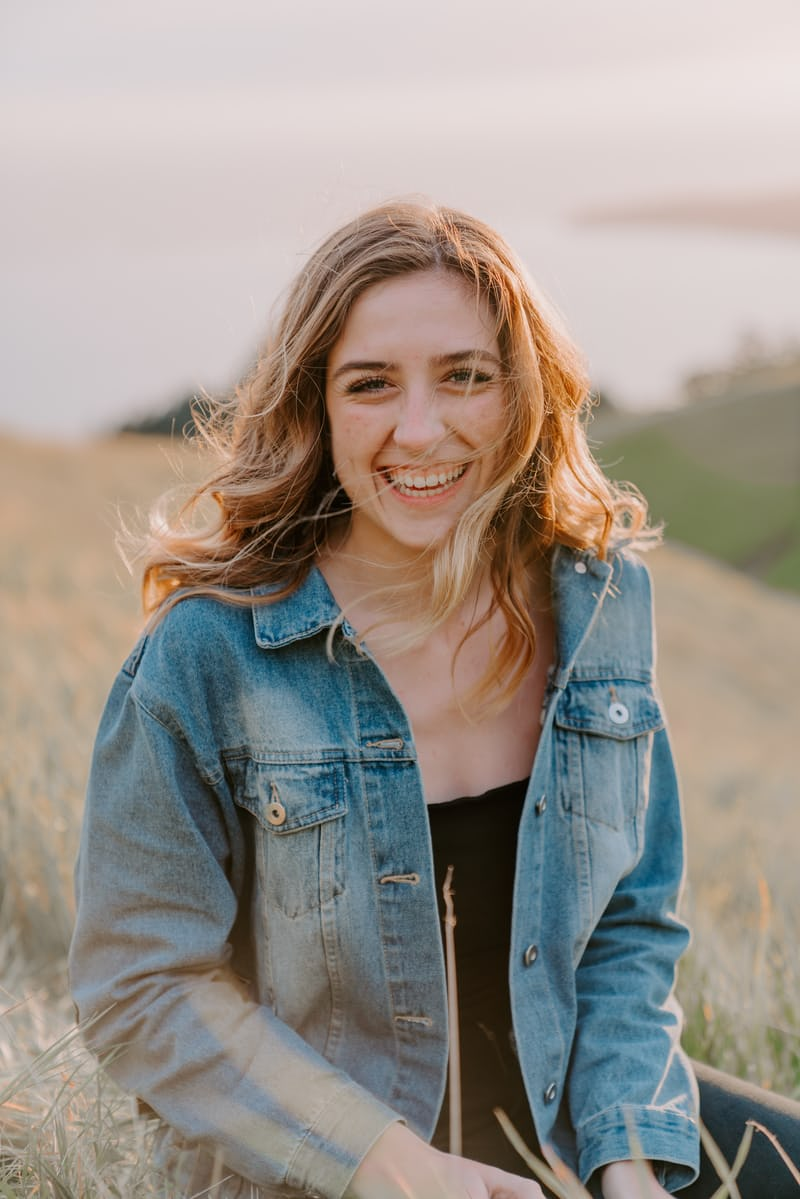
\includegraphics[angle=90,width=\textwidth]{rosa}
	\centering
	\caption{Storyboard Rosa – Als OSMI Student möchte ich Fahrgemeinschaften gründen, um mir Fahrtkosten zu sparen.}
\end{figure}

\newpage

\subsection{Storyboard 4 für Rosa Beetz}

\begin{figure}[h]
	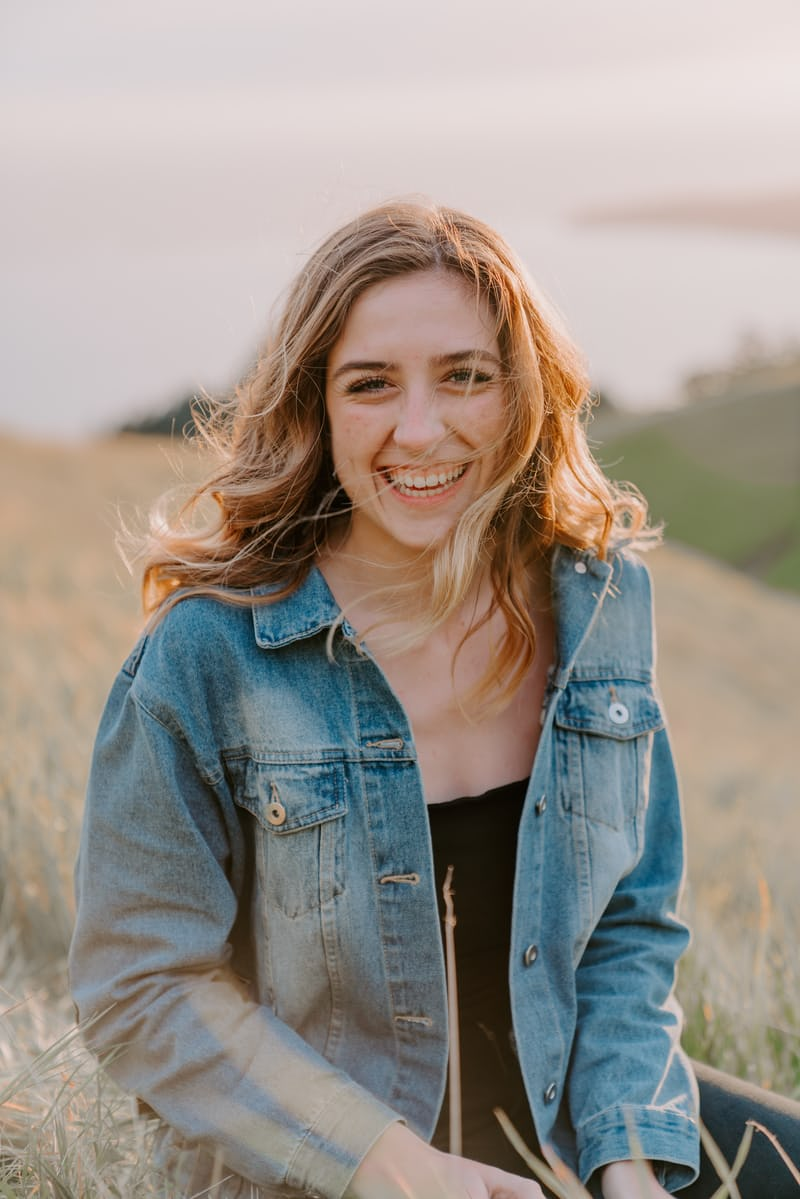
\includegraphics[angle=90,width=\textwidth]{rosa}
	\centering
	\caption{Storyboard Rosa – Als OSMI Student möchte ich mit anderen Studenten Videotelefonieren, um eine zugängliche Plattform für unsere digitale Lerngruppe zu haben.}
\end{figure}

\newpage

\section{Einsatzmöglichkeiten für Präsenzstudenten}

Foo baz

\end{document}